%TODO W Boson Masse Divergenz Theorie
%TODO Z Boson Divergenz
%TODO Higgs Boson => Masse
%TODO folie kopieren und stichpunkte repeat
\subsection{Einordnung im Standardmodell der Elementarteilchen}

\begin{iframe}
	\begin{columns}
	\begin{column}{0.48\textwidth}
		\begin{figure}
			\centering
			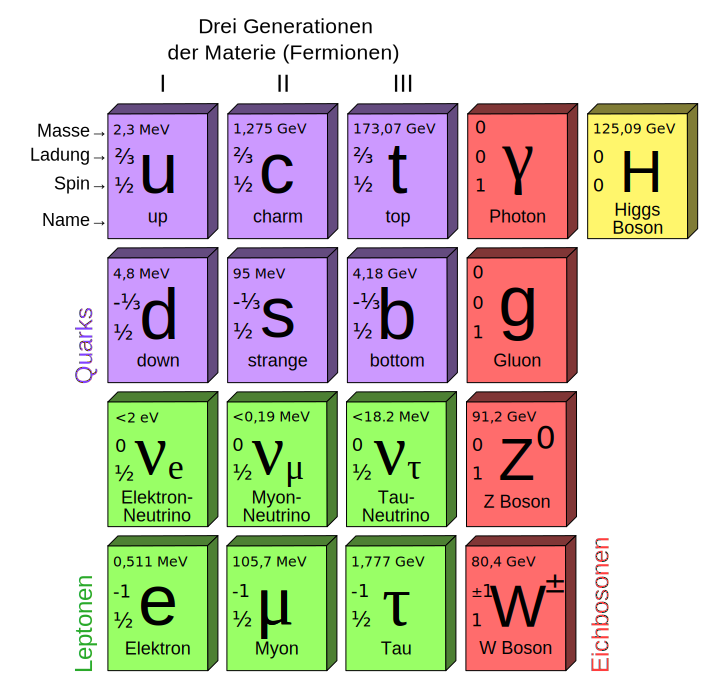
\includegraphics[width=5.5cm]{img/standardmodel}
			\caption*{Standardmodell\cite{standardmodel}}
		\end{figure}
	\end{column}
	\begin{column}{0.48\textwidth}
		$Z^0$-Boson:
		\begin{itemize}
			\item Lebensdauer $\tau\approx\SI{3e-25}{s}$
			\item Masse $M=\SI{91.2}{GeV}$
			\item ungeladen
			\item eigenes Antiteilchen
		\end{itemize}
	\end{column}
	\note[item]{Antiteilchen invers}
	\note[item]{Masse steigt mit Generation}
	\note[item]{Lebensdauer sehr sehr kurz}
	\note[item]{Masse (Reichweite)}
	\note[item]{ungleaden/neutral}
	\note[item]{Boson also Spin 1, außer Higgs}
	\note[item]{Schwache Wechselwirkung}
	\note[item]{Bestätigung der 3 Neutrinogenerationen}
\end{columns}

\end{iframe}

%\note[itemize]{
	%\item lila(Quarks), grün(Leptonen), rot(Eichbosonen), gelb(Higgs)
	%\item Generationen, Fermion , s=1/2
	%\item Boson s=1
	%\item Ladung Fermionen 2/3 -1/3 0 1  Bosonen 0 außer W \pm 1
	%\item Antiteilchen invers
	%\item
	%\item Masse steigt mit Generation
	%\item schwache WW
	%\item W+- => elek. Teilchen WW (beta Zerfall)
	%\item Z0 => auch neutral Teilchen WW (Neutrino)
%}

\subsection{Elektroschwache Vereinheitlichung}

\begin{iframe}


	\framesubtitle{Austauschteilchen}
	\begin{itemize}
		%\pause
		\item Photon $\rightarrow$ elektromagnetische Wechselwirkung
		%\pause
		\item Gluon $\rightarrow$ starke Wechselwirkung
		%\pause
		\item W-, Z-Boson $\rightarrow$ schwache Wechselwirkung
	\end{itemize}

\note[item]{Warum? Weil Divergenzen in höherer Ordnung/Energien auftreten } %TODO mehr
\note[item]{Vereint QED mit schwacher WW.}
\note[item]{ Kräfte durch Austauschteilchen}
\note[item] { Photon elektro magn. beispielweise Elektron-Elektron-Streuung, Rutherford Streuung}
\note[item]{W,Z bsplw. Beta-Zerfall, Elektron-Positron-Streuung (Energieabhänig)}
\note[item]{Gluon Kernzusammenhalt,Farbladung,8 (n-p-Anziehung), Quarkanziehung}

\note[item]{Nur durch Z-Boson lässt sich Neutrino-Neutrino-WW erklären, da sie nicht elektrisch sind.}

%\note[item]{ Allg. Grund + Was es ist.} %TODO:w

%\note[item] {?schwere Austauschteilchen => geringe Stärke der WW. (Graviton schwerer als Higgs)?} %TODO
%\note[item] {(experimentelle Bestimmung)}
%\note[item] {(Higgs)}
\end{iframe}

\begin{iframe}
	\framesubtitle{Schwacher Isospin}
	\begin{figure}
		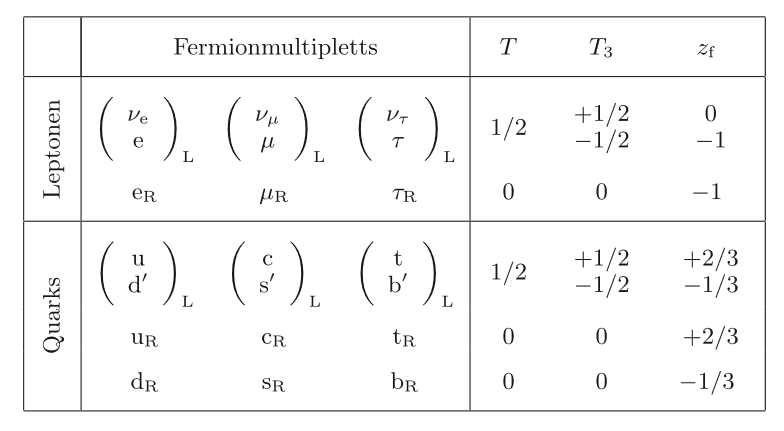
\includegraphics[height=5cm]{img/isospin}
		\caption*{Schwacher Isospin\cite{povh}}
	\end{figure}
\note[item]{ Einführung von schwachem Isospin, analogon zu starkem Isospin}
	\note[item]{ Chiralität Index R/L formal: Zerlegung von Dirac-Spinoren in orthogonale Zustände die unter Paritätsoperationen ineinander übergehen. Eigenzustände $\pm1$}
	\note[item]{ Rechtshändige $e,\mu,\tau$ Singulett Zustand.}
		\note[item]{ Chiralität (l/r), Spinor Symmetrie}
	\note[item]{ Rechtshändige  Neutrinos $T_3=z=0$, keine WW, Auftreten in Natur unbekannt }
	\note[item]{ Der ' bedeuted != Masseneigenzustände, sondern Quarkmisch-Matrix CKM }

	\note[item]{$T_3$ Werte Bereich analog zu anderen Spins}
	\note[item]{ $z_f$ beschreibt Ladung }
\note[item] {invers für Antiteilchen: rechshändige Fermionen (linkshändige Antifermionen) Singulettt ($T=0=T_3$)}
	\note[item]{ Umwandung durch Absorption von $W^\pm$-Boson innerhalb Multiplett (darin Ladungsdifferenz = 1)}
\end{iframe}
	%\item ?was bedeutet der ' (Cabibbo-Rotation)? %TODO

\begin{iframe}
	\framesubtitle{Schwacher Isospin}
	\begin{columns}
		\begin{column}{0.48\textwidth}

			\begin{overprint}
				\onslide<1>\begin{figure}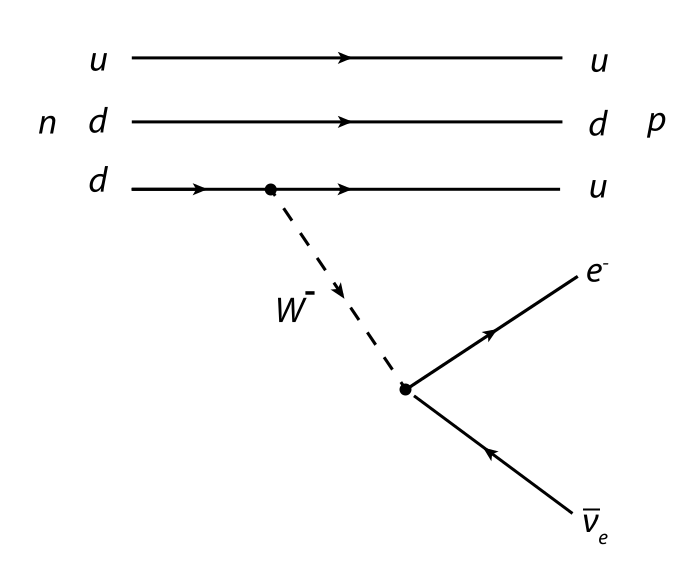
\includegraphics[height=4.5cm]{img/betadecay_old}\caption*{$\beta^-$-Zerfall\cite{beta}}\end{figure}
				\onslide<2>\begin{figure}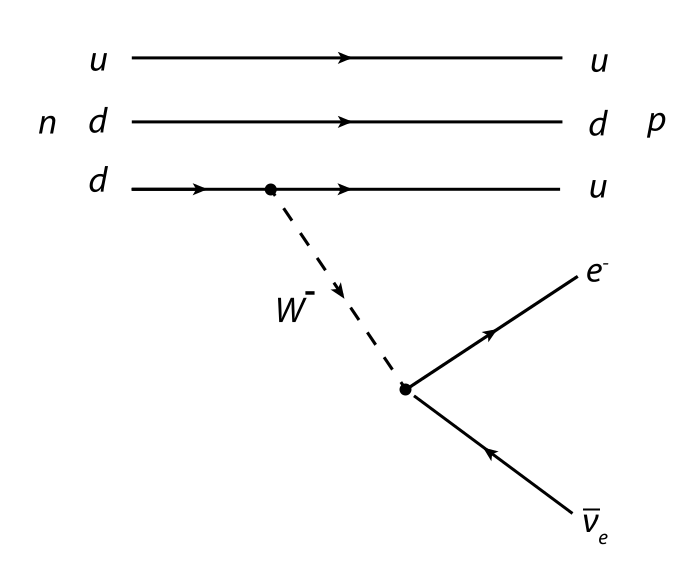
\includegraphics[height=4.5cm]{img/betadecay_old}
\caption*{$\beta^-$-Zerfall\cite{beta}}\end{figure}
				\onslide<3>\begin{figure}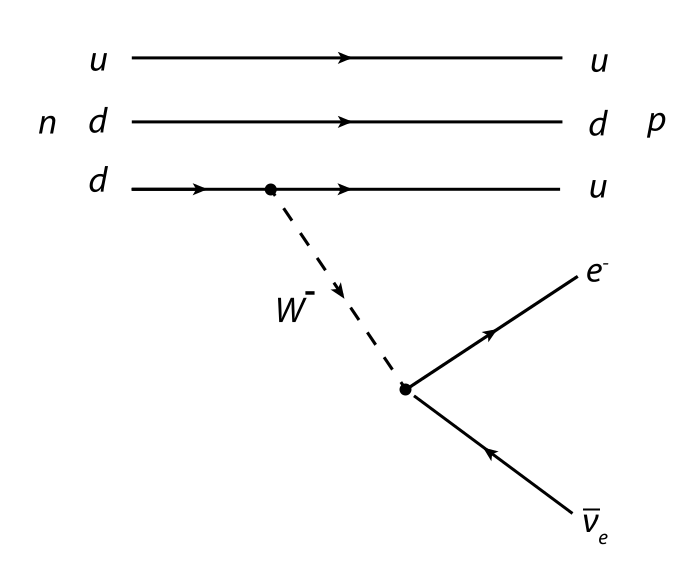
\includegraphics[height=4.5cm]{img/betadecay}
\caption*{$\beta^-$-Zerfall\cite{beta}}\end{figure}
				\onslide<4>\begin{figure}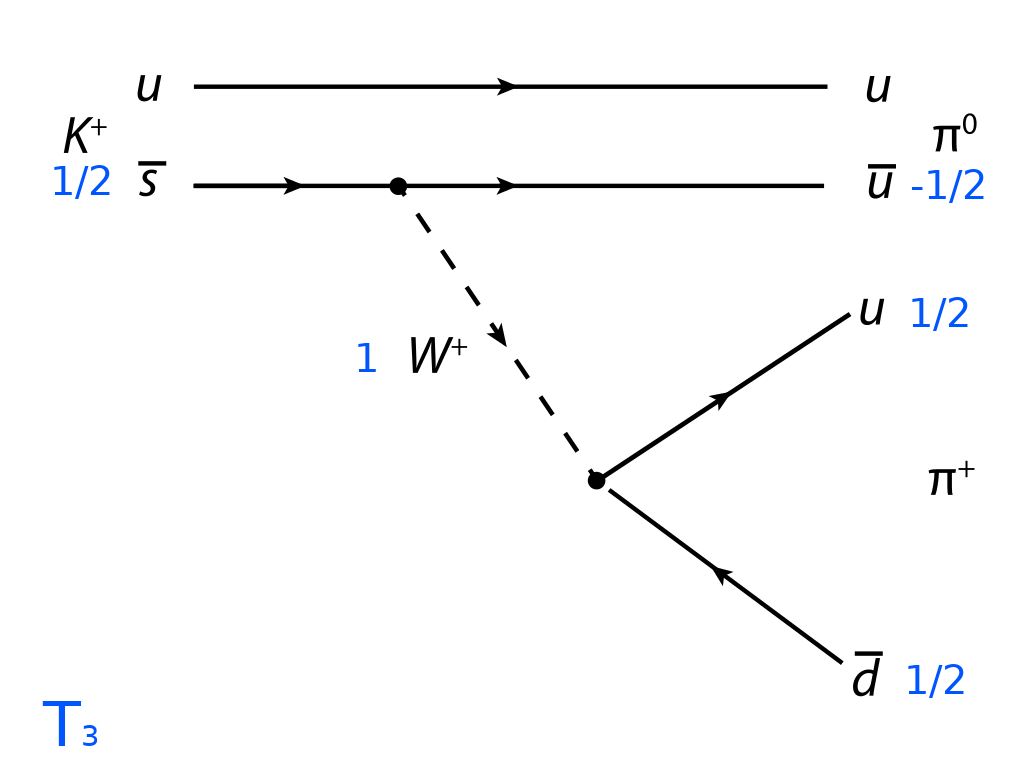
\includegraphics[height=4.5cm]{img/kaondecay}
\caption*{$K^+$-Zerfall\cite{beta}}\end{figure}
				\onslide<5>\begin{figure}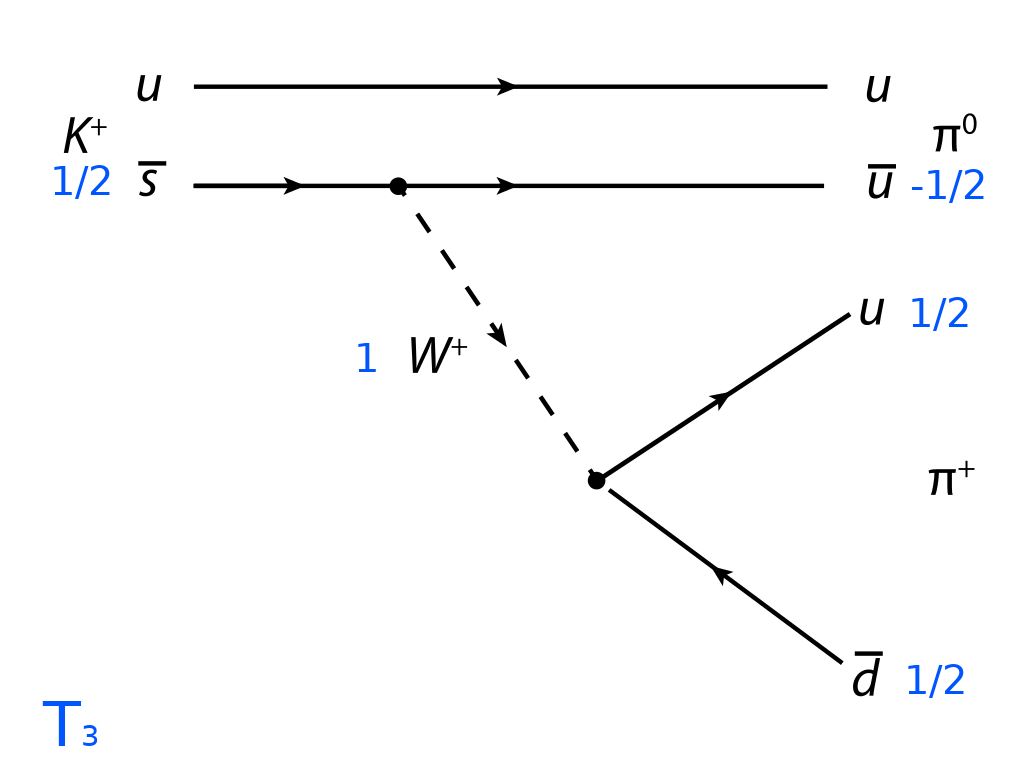
\includegraphics[height=4.5cm]{img/kaondecay}
\caption*{$K^+$-Zerfall\cite{beta}}\end{figure}
	\end{overprint}
	\end{column}
		\begin{column}{0.48\textwidth}

	\begin{itemize}
		\pause
		\item $T_3$ soll erhalten bleiben
		\pause
		\item $W^-$: $T_3=-1$
		\pause
		\item $W^+$: $T_3=1$
		\pause
		\item $W^0$: ($T=1,T_3=0$)
		\item $B^0$: ($T=0,T_3=0$)
	\end{itemize}
		\end{column}
	\end{columns}
	\only<1> {
	\note[item]{ Bekannt aus schwacher WW }
	\note[item]{ d$\rightarrow$u + $W^-$ }
	}
	\only<2> {
	\note[item]{$T_3$ Erhaltungsgröße}
	}
	\only<3> {
	\note[item]{$T_3$ in Graphik}
	\note[item]{$W^-$ muss -1 sein}
	%\note[item] {T: d(-1/2)=W(?)+u(1/2)}
	%\note[item] {T: W(?)=e(-1/2)+$\nu$(-1/2)}
	}
	\only<4> {
	\note[item]{ analog $\beta^+$-Zerfall: u$\rightarrow$d + $W^+$ }
	\note[item]{ Hier Kaon-Zerfall }
	}
	\only<5> {
	\note[item]{ Analog zu 1/2x1/2 Gekoppelten Spins}
	\note[item]{Tripplett und Singulett Zustände}
	\note[item] {$B^0$ postuliert}
	\note[item] {Mehr zum Beta-Zerfall nächste Woche (+Paritätsverletzung)}
	}
	%\note[item] {?Wieso T=1?} %TODO
\end{iframe}

\begin{iframe}
	\begin{itemize}
	\item Photon und $Z^0$ als orthogonale Linearkombination von $B^0$ und $W^0$:
		\begin{align*}
		 \ket{\gamma} &= +\cos{\theta_\text{W}} \ket{B^0} + \sin{\theta_\text{W}} \ket{W^0}	\\
		\ket{Z^0} &= -\sin{\theta_\text{W}} \ket{B^0} + \cos{\theta_\text{W}} \ket{W^0}
		\end{align*}
		\pause
	\item Weinbergwinkel:
		\begin{equation*}
		\cos{\theta_\text{W}}=\frac{M_\text{W}}{M_\text{Z}} \approx 0.88
		\end{equation*}
	\pause
		\item Gekoppelte Ladungen:
		\begin{equation*}
		e = g \cdot sin{\theta_\text{W}}
		\end{equation*}
	\end{itemize}
	\only<1> {
	\note[item]{ Drehung um Weinberg-Winkel/elektroschwachen Mischungswinkel , Naturkonstante}
	\note[item] {spontane Symmetriebrechung, diagonaliesierung der Massematrix führt zu diesen.}
	\note[item] {orthogonal + linear Kombination}
	}
	\only<2> {
	\note[item] {experimentelle Bestimmung, später mehr}
	\note[item] {Masse für $Z^0$ leichter zu Bestimmen, da W-Boson in Neutrino zerfällt. => bestimmung über fehlenden Transversalimpuls}
	}
	\only<3> {
	\note[item] {schwache Ladung g (Analogon zu e) aus schwache WW. aus QFT}
	\note[item] { beschreibbar durch elektrische und schwache Ladung}
	\note[item] {Umformung zu e/g  und M/M}
	}
\end{iframe}

%\subsection{Zerfallsbreite}
